\newcommand{\model}{%
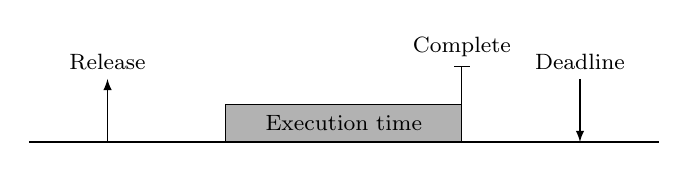
\begin{tikzpicture}[
  yscale = 0.8,
  normal/.style={fill=black!30},
  release/.style={-latex},
  complet/.style={-|},
  every text node part/.style={align=center}
]
%general params
\def\th{.6} %task height
\def\blockdim{(.4,.4)}
\def\arrowdim{(0,.5)}
\def\arrowdimB{(0,.4)}

%axes
\draw[thick, black] (0,0) -- (8, 0);

%L1
\draw[release] (1, 0) -- +(0,1) node[above] {{\footnotesize Release}};
\draw[normal]  (2.5, 0) rectangle +(3, \th) node[midway] {{\footnotesize Execution time}};
\draw[complet] (5.5, 0) -- +(0, 1.2) node[above] {{\footnotesize Complete}};
\draw[release] (7, 1) node[above] {{\footnotesize Deadline}} -- (7,0);

\end{tikzpicture}
}


\section{Introduzione}
\label{sec:introduzione}

Il continuo progresso tecnologico ha portato ad un rapido incremento della complessita del software e della richiesta di prestazioni hardware. Inizialmente per aumentare la potenza di calcolo si ricorreva a processori sempre piu' potenti, ma tale approccio a lungo andare ha portato a problematiche come l'elevato consumo di energia e l'eccessiva dissipazione di calore. Pertanto, i produttori, Intel in primis, hanno adottato piattaforme multiprocessor per lo sviluppo di sistemi real-time, quindi affiancando piu' processori piuttosto che potenziarne uno unico.\\

Burns e Wellings in ~\cite{Burns:2009:RSP:1643588} definiscono un sistema real-time come segue:\\

\textit{"an information processing system which has to respond to externally generated input stimuli within a finite and specified period. The correctness depends not only on the logical result but also on the time it was delivered. The failure to respond is as bad as the wrong response."}\\

Il cambiamento di tendenza ha spostato l'attenzione della ricerca dai sistemi single processor, per i quali lo studio e' maturo, alle piattaforme multiprocessor. Nonostate i grandi sforzi ed i recenti risultati, gli algoritmi di scheduling e le tecniche di analisi di schedulabilita' per i sistemi multiprocessor non sono ancora al livello dei precedenti single processor (Davis et al.~\cite{Davis:2011:SHR:1978802.1978814}).\\

Liu et al.\cite{Liu:1973:SAM:321738.321743} evidenziano come lo scheduling sia un problema intrinsecamente piu' complicato in ambito multiprocessor:\\

\textit{“Few of the results obtained for a single processor generalize directly to the multiple processor case; bringing in additional processors adds a new dimension to the scheduling problem. The simple fact that a task can use only one processor even when several processors are free at the same time adds a surprising amount of difficulty to the scheduling of multiple processors.”}\\

\subsection{Introduzione ai Sistemi Real-Time}
\label{sec:overviewRTS}

In questa sezione e' descritto il modello di task sporadico utilizzato e trae origine dal lavoro di Mok et al.~\cite{Sha:2004:RTS:1028913.1028959}. Tale scelta e' dettata dal fatto che il sistema LITMUS\textsuperscript{RT} e' sviluppato a partire da questo modello, mentre MrsP e' anch'esso basato su un modello sporadico senza specificarne uno in particolare. Nel proseguo del documento la nomenclatura originale subisce alcune modifiche per coerenza con il lavoro di Burns e Wellings ~\cite{Burns:2013:SCM:2547348.2547350}.

\subsubsection{Workload}
\label{sec:overviewWL}

Il \textit{workload} consiste in un insieme di $n$ task $\tau = {\tau_1, ... , \tau_n}$. Ogni task $\tau_i$ e' ripetutamente invocato in modo asicrono da un evento esterno, per esempio un \textit{interrupt} da parte di un dispositivo o lo scadere di un timer. Quando invocato esso rilascia un \textit{job} per gestire l'evento che l'ha scaturito. Il $j-esimo$ job di un task $\tau_i$ e' identificato con $J_{i,j}$ ($j \geq 1$). In casi in cui l'indice del job risulti irrilevante $J_i$ denota un qualsiasi job di $\tau_i$.\\

\paragraph{Tasks.} Ogni task $\tau_i$ e' caratterizzato da una tripla di valori:\\
\begin{itemize}
	\item $C_i$, \textit{worst case execution time} (WCET), il tempo massimo richiesto per eseguire;
	\item $T_i$, il periodo, il tempo minimo tra un evento di rilascio di un job ed il successivo;
	\item $D_i$, la dealdine, lasso di tempo a disposizione per eseguire.\\
\end{itemize}

Mentre il periodo e la deadline sono arbitrarie, il WCET dipende dalla piattaforma di esecuzione e la semantica del job. Nel primo caso dipende dalle componenti dell'hardware, per esempio la cache, la quale ha comportamenti che dipendono dalle esecuzioni precedenti che ne cambiano lo stato, o la frequenza di clock dei processori. Il secondo dipende dall'esecuzione del job, cioe' se contene istruzioni di \textit{branch} o meno, di conseguenza il flusso delle operazioni varia modificando il tempo di esecuzione. Il valore di WCET deve essere un limite massimo certo che rende il modello deterministico.\\

I valori che compongono la tripla sono soggetti ad alcuni vincoli:\\

\begin{itemize}
	\item $C_i > 0$, il tempo di esecuzione deve essere non nullo;
	\item $T_i \geq C_i$, il periodo deve essere maggiore o uguale al WCET;
	\item $D_i \geq C_i$, la dealdine deve essere maggiore o uguale al WCET.\\
\end{itemize}

\paragraph{Jobs.} Un job $J_{i,j}$ diviene disponibile per l'esecuzione al suo evento di rilascio $a_{i,j}$, con $a_{i,j} \geq 0$. La frequenza dei rilasci di un job e' determinata dal periodo del task corrispondente: $a_{i,j+1} ≥ a_{i,j} + T_i$. Ogni job $J_{i,j}$ richiede al massimo $C_i$ unita' di tempo del processore per completare la propria esecuzione entro $f_{i,j}$, con $f_{i,j} \geq a_{i,j}$. Un job si definisce in \textit{pending} dal momento di rilascio fino al suo completamento. Un task non puo' avere due job in pending allo stesso momento, quindi un job viene rilasciato solamente se il suo predecessore ha terminato la propria esecuzione. Il \textit{response time} di un job e' pari al tempo in cui rimane pending; quindi $r_{i,j} = f_{i,j} − a_{i,j}$.\\
Il modello sporadico deriva dal modello a task periodico in cui viene rilassato il vincolo che obbliga un task ad avere rilasci strettamente periodici, cioe' $ai,j = a_{i,1} + (j − 1) * T_i$; tale limite diviene un valore minimo e non un vincolo stretto.

\paragraph{Deadline.} La deadline relativa $D_i$ determina la quantita' di tempo a disposizione del job per il completamento. Il job $J_{i,j}$ deve eseguire entro la deadline assoluta $d_{i,j} = a_{i,j} + D_i$. In caso di esecuzione che termina dopo la deadline assoluta si e' in presenza di \textit{deadline miss} e comporta un ritardo del job, formalmente definita \textit{tardiness}. Una deadline miss ritarda il rilascio del successivo job.\\
La relazione tra deadline e periodo permette di categorizzare i task:

\begin{itemize}
	\item deadline implicite se $D_i = T_i$ per ogni $\tau_i \in \tau$;
	\item deadline vincolate se $D_i \leq T_i$ per ogni $\tau_i \in \tau$;
	\item deadline arbitrarie se non vi e' alcun vincolo.
\end{itemize}

La categoria di deadline ha un importante impatto sulle tecniche di analisi di schedulabilita', al contrario dal punto di vista dell'implementazione non comporta rilevanti differenze. Nel prosuguo di questo documento si assume un insieme di task con deadline implicite.\\

In figura \ref{fig:model_job} e' riassunto parte del modello discusso finora.

\begin{figure}
\centering
\model
\caption{Job del modello.}
\label{fig:model_job}
\end{figure}

\paragraph{Processor demand.} $C_i$ indica il tempo di esecuzione richiesto da ogni job di $\tau_i$, cioe' per quanto tempo il job necessita di essere assegnato ad uno dei processori per eseguire il WCET entro la deadline. In presenza di una lunga serie di job rilasciata da parte di un task e' utile normalizzare la domanda di processore mettendo in relazione periodo e deadline. Pertanto, si definisce un fattore di utilizzazione $U_i = C_i / P_i$ per ogni $\tau_i$. Tale valore e' importante in questo identifica l'ammontare di tempo in esecuzione richiesto per l'intera durata di vita del task, se tale necessita' non e' soddisfatta l'accumulo di tardiness puo' affliggere l'intero sistema.

\paragraph{Vincoli temporali.} Un sistema viene categorizzato in base ai vincoli temporali dei task che lo compongono, cioe' cosa consegue ad una deadline miss:
\begin{itemize}
	\item hard real-time, se causa un \textit{fatal fault};
	\item soft real-time, se e' indesiderabile;
	\item firm, se non diminuisce i risultati delle computazioni non sono piu' utili.
\end{itemize}

\subsubsection{Le risorse}
\label{sec:overviewRM}

Le risorse di un sistema si dividono in attive e passive. Un job necessita di una risorsa attiva per poter progredire nella propria esecuzione; esse consistono nei processori. Al contrario le risorse passive sono utilizzate dai job in quanto forniscono funzionalita', generalmente sono riutilizzabili a meno che il loro utilizzo non le esaurisca; esse sono per esempio memoria, lock e mutex.\\

L'organizzazione dei processori permette di classificare i sistemi real-time in base al loro numero ed il loro funzionamento. Sistemi con un unico processore sono definiti \textit{uniprocessor}; al contrario \textit{multiprocessor} indica sistemi con un numero di processori maggiore o uguale a due. In base alla loro configurazione un sistema multiprocessor puo' essere:

\begin{itemize}
	\item omogeneneo, i processori che lo compongono sono identici per prestazioni e caratteristiche (cache, I/O bus, set di istruzioni, etc.): il WCET di ogni job non dipende dall'unita' su cui esegue, di conseguenza sono interscambiabili;
	\item uniforme, se si differenziano per prestazioni ma hanno caratteristiche differenti: i job eseguono con tempistiche differenti sui vari processori;
	\item eterogeneo, i processori hanno differenti prestazioni e caratteristiche: non tutti i job possono eseguire su tutti i processori.
\end{itemize}

L'organizzazione dell'accesso alla memoria e le comunicazioni tra processori identifica due differenti categorie di sistemi: a memoria condivisa ed a memoria distribuita. Nel primo caso i processori condividono un'unica memoria centrale tramite un bus condiviso (architettura a sx in Figura~\ref{fig:memory}), nel secondo ogni processore (o un sottoinsieme ristretto) ha una propria memoria e comunica tramite un bus dedicato allo scambio di messaggi (dx in Figura~\ref{fig:memory}). Il sistema a memoria distribuita incombe in alti overhead in caso di migrazioni, in quanto l'intero stato del processo migrante deve essere copiato da una memoria all'altra. Al contrario, il sistema a memoria condivisa necessita di copiare solamente i registri hardware da un processore all'altro, pertanto l'operazione e' dastricamente meno onerosa.\\
Il sistema a memoria condivisa e' piu' utilizzato rispetto alla versione distribuita nonostante il bus condiviso per l'accesso alla memoria sia un collo di bottiglia in quanto l'accesso e' garantito ad un solo processo o ad un numero limitato al medesimo momento. Un sistema di questo tipo si differenzia a sua volta in due categorie in base alla gestione dell'accesso: \textit{uniform memory access} (UMA), se viene garantito uguale gestione a tutti processi, o \textit{non-uniform memory access} (NUMA), nel caso contrario.\\

Data la sua semplicita', la maggior parte dei lavori in letteratura riferiscono a sistemi multiprocessor identici con memoria condivisa ad accesso uniforme, piu' comunemente definita SMP (\textit{symmetric multiprocessor platform}). Nel proseguo del documento e' adottata tale architettura.

\begin{figure}
\includegraphics[width=\linewidth]{images/memory_arch.jpeg}
\caption{Illustrazione di architetture con memoria condivisa e distribuita.}
\label{fig:memory}
\end{figure}

\subsubsection{Scheduler}
\label{sec:overviewSCHED}

L'obiettivo di uno scheduler real-time e' di gestire l'esecuzione del sistema, quindi soddisfare le richieste dei task che compongono il workload entro i requisiti temporali. Formalmente, un algoritmo di scheduling e' un algoritmo che, dato una sequenza di job deve determinare in ogni istante quale job deve eseguire ed in quale processore. Il piano di esecuzioni risultante dall'algoritmo e' definito \textit{schedule}. Un algoritmo per essere valido deve rispettare i seguenti vincoli:\\

\begin{itemize}
	\item in ogni istante ad ogni processore e' assegnato al massimo un job 
	\item in ogni istante un job e' assegnato al massimo ad un processore
	\item un job non e' eseguito fino al momento del suo rilascio
	\item la quantita' di tempo del processore assegnata ad ogni job e' al massimo pari al suo WCET
	\item un job esegue su un processore per volta.
\end{itemize}

Un algoritmo si definisce corretto se produce uno schedule valido. A sua volta uno schedule e' definito \textit{feasible} se ogni job esegue entro la propria deadline. Un taskset e' \textit{schedulable} in relazione ad un algoritmo di scheduling se produce uno schedule feasible, pertanto e' una proprieta' che dipende dal taskset e non dipende dall'algoritmo. Al contrario, un algoritmo e' ottimo se genera sempre uno schedule feasible dato un qualsiasi taskset feasible.\\

Un test di schedulabilita' determina se un algoritmo genera uno schedule feasible se applicato ad un particolare taskset, esso puo' essere sufficiente o necessario: nel primo caso un esito negativo indica un taskset non feasible, nel secondo caso un risultato positivo indica un taskset feasible. Un test che e' sia sufficiente che necessario e' definito esatto.\\

\subsection{Real-time scheduling in sistemi multiprocessor}
\label{sec:SchedMulti}

Lo scopo dello scheduler e' quello di selezionare ad ogni evento di scheduling un job dalla coda ready, quindi da quelli in attesa di eseguire.L'organizzazione e la gestione di tale coda permette di differenziare gli scheduler in base a diverse caratteristiche.\\

I sistemi in cui e' presente un unica coda sono definiti globali: le esecuzioni su tutti i processori sono gestite prelevando i job da un'unica coda, essi possono di conseguenza eseguire su tutti i processori in modo indistinto. Al contrario in un sistema partizionato i task sono suddivisi ed allocati ognuno in un unico processore, di conseguenza vi e' una coda per ogni processore sulla quale lo scheduler opera. Una versione ibrida tra i due sistemi prevede che i processori siano divisi in sottoinsiemi e per ognuno di essi vi sia un'unica coda, tale configurazione prende il nome di scheduler a \textit{cluster}.\\

L'ordinamento della coda avviene in base alla proprieta', la modalita' di assegnazione di tale valore ai job permette di distinguere gli algoritmi:

\begin{itemize}
	\item task a priorita' fissa: ad ogni task e' assegnata una certa priorita' che viene applicata ad ogni job che rilascia;
	\item job a priorita' fissa: i job del medesimo task possono avere priorita' differente, ma ogni job ha un'unica priorita'; un esempio e' \textit{Earliest Deadline First} (EDF)
	\item priorita' dinamica: la priorita' di un job puo' assumere differenti valori, per esempio \textit{Least Laxity First} (LLF).
\end{itemize}

L'approccio partizionato e' largamente utilizzato in quanto ogni singola partizione puo' essere analizzata ed eseguita come un sistema single processor, con i relativi vantaggi dati da uno studio di tecniche ed algoritmi maturi. Nonostante questo ha lo svantaggio di dipendere dalla fase offline di allocazione dei task tra i processori; tale problema e' riportabile al ben piu' noto \textit{bin-packing}. Esso e' uno dei problemi classici dell'informatica ed e' NP-hard (Garey et al.~\cite{Garey:1979:CIG:578533}). Di conseguenza l'intero sistema dipende dalla risoluzione di tale problema, conducendo quindi ad una soluzione al di sotto delle effettive prestazioni della piattaforma utilizzata dato che non si raggiunge un fattore di utilizzazione vicino all'ottimo. Oltre a questo svantaggio, la condivisione di risorse tra task allocati in differenti processori causa un negativo impatto alla schedulabilita' del taskset. Al contrario un sistema globale garantisce un alto livello di utilizzazione, ma comporta alti valori di overhead dati dalla gestione di un'unica coda.\\

Davis et al.~\cite{Davis:2011:SHR:1978802.1978814} propone una panoramica dei principali scheduler in sistemi partizionati, clustered e globali. Il proseguo del documento si focalizza su sistemi partizionati con utilizzo di task a priorita' fissa.\\

\subsection{Real-Time Locking Protocols}
\label{sec:lockProtocols}

Il sistema descritto nella Sezione~\ref{sec:overviewRTS} assume che i task siano indipendenti, cioe' che non condividano risorse diverse dal processore stesso. In un sistema a task indipendenti, gli \textit{m} job ready con priorita' maggiore (con \textit{m} pari al numero di processori) eseguono. I job proseguono fino al loro completamento ogni qual volta gli sia assegnato un processore. Molti degli algoritmi di scheduling studiati e le tecniche di analisi di schedulabilita' sono basati su un sistema di questo tipo. Tuttavia, in un sistema reale i task condividono delle risorse, basti pensare a dispositivi di I/O, buffer, strutture dati, etc. I task non risultano piu' indipendenti, il progredire della loro esecuzione dipende dai job con cui condividono delle risorse.\\

La condivisione di risorse necessita di meccanismi di sincronizzazione per prevenire situazioni di inconsistenza. Questa necessita' e' soddisfatta tramite l'utilizzo di \textit{lock}: il job richiede una risorsa, se in uso attende il suo rilascio, una volta libera ne acquisisce il possesso. Potenzialmente, questo funzionamento preclude l'avanzamento dell'esecuzione nonostante sia assegnato ad un processore. Sono possibili altri approcci definiti \textit{non-blocking} che permettono al job di non attendere, ma tali protocolli sono molto onerosi per quantita' di memoria richiesta o overhead che comportano.\\

In un sistema singleprocessor un job che richiede una risorsa occupata puo' solamente sospendersi in attesa del suo rilascio, in caso contrario il possessore non potrebbe portare a termine la sezione critica (cioe' la parte di esecuzione che richiede l'uso della risorsa e che necessita di sincronizzazione) causando cosi' stallo nell'intero sistema. Le circostanze in cui un job a priorita' inferiore esegue a discapito di uno a priorita' superiore a causa della condivisione di risorse e' chiamta \textit{inversione di priorita'}. Uno degli obiettivi principali di un protocollo di accesso a risorsa e' quello di limitare tale inversione in quanto rende complesso effettuare un test di schedulabilita', oltre che snaturare il normale flusso dell'esecuzione in cui un job a priorita' superiore esegue prima di uno a priorita' inferiore. In un sistema multiprocessor il job puo' sospendersi, come nel caso precendete, o effettuare attesa attiva fino al suo rilascio. [grafico con due job, uno esegue l'altro attende]. L'utilizzo di attesa attiva ha lo svantaggio di sprecare l'esecuzione del processore, ma ha il vantaggio di essere di semplice implementazione e causa basso overhead; al contrario la sospensione, tra i vari svantaggi, causa allungamento nel tempo di blocco subito da parte del job che richiede la risorsa. Per uno studio dettagliato della gestione del caso di blocco da parte di un job si veda Brandenburg et al.~\cite{Brandenburg:2008:RSM:1440456.1440601}.\\

Un protocollo di accesso di risorsa deve garantire che i ritardi causati agli altri job siano limitati e calcolabili con precisione ed allo stesso tempo i job a priorita' superiore non devono subire ritardi da job con cui non condividono risorse. Questo problema e' stato risolto in ambito singleprocessor con i protocolli PIP, PCP e SRP (Sezione~\ref{sec:lockProtocols.single}). Altrettanto non si puo' dire per i sistemi multiprocessor per i quali la maggior parte dei protocolli risolvono il primo problema, cioe' quello di limitare il ritardo per i job, ma senza garantire indipendenza ai job a priorita' superiore (Sezione~\ref{sec:lockProtocols.multi}). Al contrario OMIP (Sezione~\ref{sec:lockProtocols.omip}) e MrsP (Sezione~\ref{sec:lockProtocols.mrsp}), con approcci differenti, garantiscono sia blocco ridorto che l'indipendenza dei job a priorita' superiore.\\

\subsection{Singleprocessor Protocols}
\label{sec:lockProtocols.single}

I protocolli per piattaforme con un unico processori sono stati ampiamenti studiati, in particolare sono presenti test di schedulabilita' per FP e EDF che considerano l'inversione di priorita' tra job data dalla condivisione di risorse.\\

\paragraph{Non-preemptive critical section protocol (NPC).} Il modo piu' semplice per limitare il tempo di blocco causato dall'inversione di priorita' e' quello di inibire il prerilascio durante la sezione critica. Pertanto il job che richiede ed ottiene la risorsa non viene prerilasciato da job a priorita' superiore fino a che non porta a termine l'esecuzione della risorsa. NPC ha il vantaggio di essere facilmente implementabile e comporta bassi livelli di overhead, in particolare per task a livello kernel in quanto e' sufficiente disabilitare gli \textit{interrupt}.\\
Il blocco subito da un job a priorita' superiore che richiede la risorsa occupata nel caso peggiore e' pari alla lughezza della sezione critica stessa ed avviene solamente una volta, precisamente prima dell'inizio della sua esecuzione. Ne consegue che NPC e' facilmente integrabile nei test di schedulabilita'. Lo svantaggio e' che causa blocco anche ai job che non condividono la risorsa.\\

\paragraph{Priority inheritance protocol (PIP).} Sha et al.~\cite{Sha:1990:PIP:102822.626613} propone un protocollo che mira a non causare blocco a job priorita' superiore che non accedono la risorsa. La particolarita' del protocollo e' che viene innescato solamente nei casi in cui il job che detiene la risorsa causa inversione di priorita', in tal caso la priorita' del job viene innalzata al valore massimo tra tutti i job in attesa in quel determinato istante. Tale protocollo ha lo svantaggio che, in determinate circostanze, conduce a deadlock.\\

\paragraph{Priority-ceiling protocol (PCP).} Sha et al.~\cite{Sha:1990:PIP:102822.626613} presenta un protocollo disegnato principalmente per algoritmi FP e risolve il problema di deadlock del protocollo precedente. Ad ogni risorsa e' abbinato un ceiling pari alla priorita' massima tra tutti i job che durante l'esecuzione la richiedono, inoltre e' previsto un ceiling di sistema pari al ceiling piu' alto tra tutte le risorse in uso in un determinato momento. La richiesta di accesso da parte di un job e' soddisfatta solamente se la sua priorita' e' superiore al ceiling di sistema; una volta ottenuta la risorsa, se nesessario, il ceiling di sistema viene innalazato. Questo meccanismo di ceiling garantisce che una richiesta di un job venga soddisfatta solamente se tutte le risorse di cui potrebbe necessitare sono al momento libere.\\

\paragraph{Stack resource policy (SRP).} Il protocollo delineato da Baker~\cite{Baker:1991:SSR:113595.113601} e' anch'esso basato su un sistema di ceiling. Ad ogni risorsa e' abbianto un ceiling, inoltre e' presente un ceiling di sistema, entrambi calcolati e gestiti secondo le indicazioni di PCP. La differenza sostanziale sta nel fatto che ad un job non e' permesso di eseguire fino a che la sua priorita' non e' superiore al ceiling di sistema, il comportamento che ne consegue e' che un job esegue solamente se tutte le risorse di cui potrebbe necessitare sono libere. Pertanto il job subisce l'inversione di priorita' solamente una volta e prima dell'inizio della sua esecuzione. SRP e' alla base del protocollo studiato in questo elaborato per le sue proprieta' fondamentali:

\begin{itemize}
\item un job e’ bloccato al massimo una volta durante la sua esecuzione;
\item tale blocco avviene prima dell’inizio dell’effettiva esecuzione;
\item quando il job inizia ad eseguire, tutte le risorse di cui necessita sono logicamente libere;
\item previene situazioni di deadlock.
\end{itemize}

\subsection{Multiprocessor Protocols}
\label{sec:lockProtocols.multi}

Nei sistemi multiprocessor le risorse sono distinte in due categore: locali e globali. Nel primo caso i task che la richiedono sono tutti allocati nel medesimo processore, quindi possono essere utilizzati protocolli di accesso tipici di sistemi singleprocessor. Al contrario, nel secondo caso la risorsa e' richiesta da job che eseguono su differenti processori.\\

I primi protocolli per sistemi multiprocessor sono il frutto di un riadattamento di protocolli singleprocessor. Se in presenza di un unico processore la serializzazione degli accessi e' intrinseca del fatto che esista un unico luogo di esecuzione, con un maggior numero di processori gli accessi sono potenzialmente paralleli, di conseguenza sono necessari meccanismi che permettano ai vari riadattamenti di soddisfare questa necessita'.\\

Un altra problematica derivante dal fatto che job su processori differenti condividono un'unica risorsa sta nel fatto che non ha senso comparare le loro proprieta': un job con la priorita' piu' alta nel proprio processore potrebbe essere meno urgente rispetto ad uno in un altro processore. I primi protocolli sviluppati per la condivisione di risorse globali ovviano a tale problema tramite il \textit{boosting} del job, cioe' innalzando la priorita' del job al di sopra di tutte le priorita' di base degli altri job. La differenza sostanziale tra la tecnica di boosting e l'inibizione del prerilascio sta nel fatto che tra \textit{job boosted} avvengono prerilasci. Le richieste vengono poi gestite in base all'arrivo (FIFO) o tramite code ordinate secondo la priorita' di base.

\subsubsection{DPCP e MPCP}
\label{sec:lockProtocols.dpcp.mpcp}

Le prime versioni derivano da un adattamento di PCP, nonostante un approccio molto simile essi si differenziano in quanto sono stati studiati per architetture differenti: in sistemi con memoria distribuita ogni risorsa e' accessibile solamente da un determinato processore nel quale e' allocata, al contrario in presenza di memoria condivisa la risorsa e' accessibile da ogni processore.\\

\paragraph{Distribuited priority-ceiling protocol (DPCP).} Rajkumar~\cite{Rajkumar:1991:SRS:532621} utilizza RPC \textit{remote procedure call} per gestire gli accessi alla risorsa: la richiesta viene presa in carico da parte di un agente locale al processore della risorsa che esegue in modo sincrono ed il job si sospende fino a che la richiesta non viene portata a termine. La priorita' del richiedente resta invariata mentre viene aumentata quella dell'agente: assumendo che $i$ sia l'indice del job richiedente, la priorita' dell'agente e' pari ad $n - 1$ ($n$ pari al numero totale di task nel sistema). L'indice e' assegnato ai job in ordine di priorita' effettiva, in questo modo i prerilasci tra gli agenti rispecchiano le priorita' dei task che li attivano. Gli agenti locali sono gestiti in base al protocollo PCP. Questo tipo di approccio causa diversi tipi di blocco in cui incorrono i job nei vari processori e gli agenti nel processore di sincronizzazione rendendo cosi' i test di schedulabilita' particolarmente pessimistici.\\

\paragraph{Multiprocessor priority-ceiling protocol (MPCP).} [NON SONO RIUSCITO A TROVARE IL BIBTEX DEL PAPER] E' un'evoluzione del precedente protocollo, progettato per sistemi con memoria condivisa. Le risorse globali possono essere accedute da ogni processore, pertanto non vi e' piu' bisogno dell'utilizzo di agenti. Una volta ottenuto l'accesso ad una risorsa il job innalza la propria priorita' a quella piu' alta tra tutti i task che la richiedono. Questo tipo di \textit{priority boosting} velocizza l'esecuzione della sezione critica diminuendo l'ammontare di inversione di priorita' subita dai job che condividono la risorsa o a priorita' inferiore al "ceiling", tuttavia senza creare blocco ai job con priorita' superiore al ceiling globale. Dato che le priorita' non sono uniche, a parita' di valore non viene permesso il prerilascio, in questo modo non si ritarda l'esecuzione della sezione critica.\\
Anhce in questo caso i job che richiedono una risorsa occupata incorrono in diversi tipi di blocco in quanto l'accesso e' garantito in base alla priorita', permettendo quindi ad altri job di accedere prima anche se l'hanno richiesta successivamente. Inoltre il blocco generato da altri job che non richiedono la risorsa potenzialmente possono ritardare l'esecuzione da parte del job in testa alla coda, causando cosi' ulteriori ritardi al job stesso ed agli altri in attesa.\\

MPCP, come DPCP, soffre di ritardi aggiuntivi derivanti dall'auto sospensione da parte dei job in attesa della risorsa. Lakshmanan et al.~\cite{5368127} propone una versione di MPCP che prevede "virtual spinning", da cui MPCP-VS. Il protocollo rivisitato dispone che il job si auto sospenda, ma che nessun altro job del medesimo processore con priorita' inferiore possa accedere ad una risorsa globale.\\

-----------------------------------------------------------------------------------------------------

\subsubsection{MSRP}
\label{sec:lockProtocols.msrp}

Gai~\cite{Gai:2003:CMM:827266.828537} propongono un riadattamento del protocollo singleprocessor SRP, da cui \textit{Multiprocessor SRP}, anche se quest'ultimo non e' utilizzato per le risorse globali, bensi' per quelle locali. La gestione dell'accesso alle risorse globali e' gestito tramite inizibizione del prerilascio: un job quando effettua la richiesta inibisce il prerilascio e, se la risorsa e' occupata, si accoda nella coda FIFO della risorsa corrispondente effettuando attesa attiva sino al raggiungimento della testa; una volta acquisita esegue la sezione critica senza permettere ai job a priorita' piu' alta del medesimo processore di eseguire. Nella Sezione~\ref{sec:lockProtocols.single} e' stato discusso come un approccio di questo tipo abbia vantaggi e svantaggi: l'attesa attiva comporta spreco di esecuzione del processore e causa blocco ai job a priorita' piu' alta che non condividono la risorsa, d'altro canto limita tale tempo di blocco al massimo alla lunghezza di un'unica sezione critica; l'attesa da parte dei job in coda per la risorsa e' delimitata alla lunghezza della FIFO, cioe' all'esecuzione dei job che lo precedono. Inoltre, dato che solamente un job alla volta per ogni processore puo' effettare una richiesta la lunghezza di coda FIFO e' al massimo pari al numero di processori. Le dinamiche appena descritte si rispecchiano nei test di schedulabilita' del protocollo, i quali permettono di limitare con precisione i costi aggiuntivi indotti dalla risorsa globale.

\subsubsection{FMLP}
\label{sec:lockProtocols.fmlp}

Block in ~\cite{Block:2007:FRL:1306877.1307316} propone un protocollo (\textit{flexible multiprocessor locking protocol} combina i due differenti approcci suspensione-based e spin-based: le risorse sono suddivise tra "brevi" e "lunghe" in relazione alla durata della sezione critica, le prime sono gestite tramite accodamento FIFO ed inibizione di prerilascio mentre nel secondo caso tramite protocollo che prevede sospensione. Le risorse definite "brevi" si presuppone abbiano una durata tale per cui l'utilizzo di altri meccanismi diversi dall'inibizione del prerilascio, che a livello kernel e' implementato in modo molto efficiente, comportino un overhead superiore rispetto al beneficio apportato. Al contrario per le risorse "lunghe" i job in attesa del suo rilascio si sospendono in modo tale da non creare ritardi agli altri job, in particolare quelli a priorita' superiore che non la accedono. Oltre ad essere utilizzabile sia in con scheduler globali che partizionati, questo protocollo permette accumulo di risorse tramile l'utilizzo di "Group locks": risorse innestate creano un unico gruppo al quale i job accedono in mutua esclusione, in tal modo una volta ottenuto il lock sull'intero gruppo e' garantito che le altre risorse di cui necessita sono libere. Quest'ultimo approccio ha pero' il difetto di penalizzare il parallelismo in quanto un job non permette di accedere delle risorse che potenzialmente non utilizza ma che fanno parte del medesimo gruppo.\\

\subsubsection{Helping protocol}
\label{sec:lockProtocols.help}

Con \textit{Helping protocol} si identifica quell'insieme di protocolli in cui un job puo' prendersi carico dell'esecuzione della sezione critica, corrispondente ad una risorsa, per conto di un altro job. Nei protocolli discussi nei paragrafi precedenti e' emerso che l'aspetto cruciale sia come gestire l'esecuzione delle sezione critica: inibendo il prerilascio si danneggiano i job a priorita' superiore che non la accedono, ma in questo modo il tempo di blocco e' limitato al tempo di utilizzo della risorsa; al contrario un innalzamento di priorita' ad un valore precalcolato comporta la possibilita' di essere prerilasciati, di conseguenza il blocco subito dagli altri job in attesa o a priorita' inferiore a tale valore aumenta. Questa categoria di protocolli prevede che l'avanzamento della sezione critica possa essere presa in carico da parte di uno dei job accodati qualora il suo detentore venga prerilasciato, pertanto l'esecuzione della risorsa viene portata a termine da un altro job ed il relativo risultato viene messo a disposizione del detentore al momento del suo risveglio. Tramite questo meccanismo il tempo di blocco e' al massimo pari alla lunghezza della sezione critica senza intaccare l'esecuzione dei job a priorita' superiore.\\

SPEEP (\textit{Spinning Processor Executes for Pre-empted Processor} di Takada et al.~\cite{641276}) si basa sull'assunzione che l'operazione corrispondente alla risorsa sia atomica: i job che la necessitano accodano la propria richiesta nella corrispondente FIFO ed essa viene presa in carica dal primo job nella coda che non e' stato prerilasciato. Il limite di tale protocollo e' appunto l'assunzione di partenza, cioe' che la sezione critica sia atomica e quindi facilmente eseguibile da ogni job in coda.\\

Faggioli at el.~\cite{5562902} propongo il protocollo \textit{Multiprocessor Bandwidth Inheritance Protocol} (M-BWI), il quale descrive un approccio differente e maggiormente complesso: i task eseguono all'interno di server, ad essi e' abbinato una quantita' di tempo per eseguire i job ed una volta averlo esaurito si sospende fino al rinnovo di tale \textit{budget}. I job che richiedono la risorsa effettuano busy-wait, senza inibire il prerilascio, fino a che non ne ottengono l'accesso, il quale e' garantito in ordinamento FIFO. I job che attendono il rilascio utilizzano il budget del proprio server per effettuare attesa attiva oppure lo possono cedere al detentore della risorsa nel caso in cui esso venga prerilasciato. Ne consegue che, al contrario di SPEEP, il job non prende in carico l'esecuzione per conto del job prerilasciato, bensi' gli cede l'esecuzione nel proprio processore per una quantita' di tempo pari al budget residuo.\\

\subsection{$O(m)$ Independence-preserving Protocol}
\label{sec:lockProtocols.omip}

OMIP è un protocollo studiato per sistemi con algoritmi clustered ed il suo obiettivo è quello di limitare il tempo di blocco subito dai job in attesa della risorsa e quelli che ne subiscono interferenza.  Brandeburg in ~\cite{6602109} dimostra come non sia possibile ottenere un limitato tempo di blocco e preservare l’indipendenza dei job a priorità superiore senza permttere migrazioni tra cluster. Brevemente, Brandeburg si sofferma sul concetto di \textit{independence-preserving}, secondo il quale i job che non accedono la risorsa non ne subiscono blocco: un job subisce blocco per un tempo pari alla lunghezza della sezione critica se la accede, zero altrimenti.\\

Il protocollo e' basato su un approccio suspension-based, pertanto un job che non riesce ad ottenere la risorsa si accoda e lascia l’esecuzione nel processore ai job a priorità inferiore. Indichiamo con $W_i$ l'insieme di job in attesa che $J_i$ rilasci la risorsa globale. Permettendo \textit{migratory priority inheritance}, ogni qual volta che $J_i$ non è in esecuzione nonostante sia ready ed esiste un job $J_x \in W_i$ tale che $J_x$ è tra i $c$ job a priorità più alta nel suo cluster, $j_i$ migra nel cluster di $J_x$ e ne eredita la priorità, causando prerilascio al job con la priorità più bassa tra quelli in esecuzione. Dopo il rilascio della risorsa, se necessario, $J_i$ migra al proprio cluster.\\
L'idea alla base è quella di far migrare il job che detiene la risorsa ogni qual volta che viene prerilasciato scegliendo un cluster tra quelli in cui vi è un job in attesa e potenzialmente in esecuzione.\\

Il protocollo utilizza una serie di accodamenti:

\begin{itemize}
\item una coda ad ordinamento FIFO abbinata alla risorsa globale, essa ha lunghezza massima pari al numero di cluster del sistema ed il job in testa alla coda ha accesso alla risorsa;
\item una coda FIFO per ogni cluster per ogni risorsa, essa ha lunghezza limitata pari al numero di processori nel cluster; il job in testa alla coda viene inserito nella coda globale;
\item una coda a priorità è apposta a quella del punto precedente.
\end{itemize}

Il funzionamento alla base prevede che una richiesta venga accodata nella coda FIFO del proprio processore e non appena raggiunge la testa passa alla coda globale. Nel caso in cui la prima coda sia piena, la richiesta viene accodata nella coda a priorità. Questo sistemi ad accodamenti preserva l'indipendenza dei job e limita il tempo di blocco.

\subsection{Multiprocessor Resource Sharing Protocol}
\label{sec:lockProtocols.mrsp}

Burns and A.J. Wellings in ~\cite{Burns:2013:SCM:2547348.2547350} delineano delle caratteristiche che un protocollo di accesso a risorsa per sistemi multiprocessor dovrebbe avere. I meccanismi che combinano hanno come obiettivo quello di creare un protocollo che permetta l’utilizzo di tecniche di analisi di schedulabilita’ tipiche di sistemi singleprocessor nelle quali si rifletta la necessita’ di serializzare le richieste di accesso alla risorsa globale, le quali sono potenzialmente parallele.\\

Il modello adottato e’ quello a task periodici approfondito in Sezione~\ref{sec:overviewWL}. $n$ task ($\tau_i$), caratterizzati da periodo $T_i$ , deadline $D_i$ e WCET, che generano una sequenza potenzialmente infinita di job. Ad ogni task e’ abbinato un valore di priorita’ $Pri(\tau_i)$. La piattaforma di esecuzione consiste in $m$ processori identici ($p_1 … p_m$).\\
Una risorsa $r$ e’ condivisa da un insieme di task. Essi devono accedere in mutua esclusione ed il codice corrispondente e’ definito \textit{sezione critica}. Definiamo la funzione $G(r_j)$, la quale ritorna l’insieme di task che utilizzano la risorsa $r_j$, e $F(\tau_i)$, per ottenere l’insieme di risorse utilizzate da $\tau_i$ . Per semplicita’ di esposizione, si assume che il tempo di esecuzione di una risorsa sia identico per ogni task ed e’ indicato da $c_j$. Inoltre, la funziona $map$ dato un insieme di task ritorna i processori in cui sono allocati.\\
Infine, definiamo $e_j$ come un parametro di tempo di esecuzione di $r_j$:\\

\centerline{$e_j = | map(G(r_j)) | * c_j$.}

Intuitivamente, $e_j$ indica il tempo massimo richiesto da un job per ottenere ed eseguire una risorsa, il quale tiene conto dello smaltimento delle richieste gia’ in coda e l’esecuzione da parte del job stesso.\\

L’approccio proposto e’ un’estensione di PCP/SRP atta a gestire gli accessi alla risorsa in un sistema partizionato con scheduler fixed priority. Ad ogni risorsa e' abbinato un insieme di ceiling, uno per ogni processore: ogni valore e' pari alla priorita' massima tra i job che la richiedono e sono allocati nel medesimo processore.\\
MrsP eredita le caratteristiche di SRP (Sezione~\ref{sec:lockProtocols.single}):

\begin{itemize}
\item un job e’ bloccato al massimo una volta durante la sua esecuzione;
\item tale blocco avviene prima dell’inizio dell’effettiva esecuzione;
\item quando il job inizia ad eseguire, tutte le risorse di cui necessita sono libere o non sono in uso nel processore corrente;
\item impedisce deadlock.
\end{itemize}

Il protocollo ha l’obiettivo di riutilizzare la tecnica di analisi di schedulabilita' singleprocessor \textit{Response-Time Analysis} (RTA) ~\cite{Audsley93applyingnew} che incorpora PCP/SRP:\\

\centerline{$R_i = C_i + max$\{\textcolor{red}{$\hat{c}$}$,\hat{b}\} + \sum\limits_{\tau_j \in hp(i)} \ceil{\frac{R_i}{T_j}} C_j$}

\vspace{4 mm}

Il secondo termine identifica il tempo di blocco subito dal job causato dalla condivisione di risorse tra job a priorita’ inferiore con job a priorita’ superiore dal quale eredita la priorita’. $C_i$ rappresenta il WCET piu’ le sezioni critiche corrispondenti alle risorse di cui necessita durante l’esecuzione ($n_i$ indica il numero di volte che $\tau_i$ utilizza $r_j$):\\

\centerline{$C_i = WCET_i + \sum\limits_{r^j \in F(\tau_i)} n_i \textcolor{red}{c^j}$}

\vspace{4 mm}

Il passaggio da un protocollo di acceso a risorsa da un sistema singleprocessor ad uno multiprocessor comporta una scelta tra limitare il tempo di interferenza agli altri job causato dalle richieste parallele ed un aumento nel tempo richiesto per accedere la risorsa. Di conseguenza si necessita di fare delle scelte algoritmiche che permettano di utilizzare le equazioni viste precedentemente aumentando il costo relativo all’accesso alle risorse.\\

MrsP incorpora la proprieta’ fondamentale di PCP/SPR, cioe’ che le risorse di un job quando inizia ad eseguire sono logicamente libere, ma l’esecuzione della risorsa non e’ pari ad una singola sezione critica $c_j$, bensi’ $e_j$.\\

Le equanzioni risultano quindi le seguenti:\\

\centerline{$R_i = C_i + max$\{\textcolor{red}{$\hat{e}$}$,\hat{b}\} + \sum\limits_{\tau_j \in hp(i)} \ceil{\frac{R_i}{T_j}} C_j$}

\centerline{$C_i = WCET_i + \sum\limits_{r^j \in F(\tau_i)} n_i \textcolor{red}{e^j}$}

\vspace{4 mm}

Per ottenere questo, MrsP prevede che una volta che un job effettua una richiesta esso continui la propria esecuzione, cioe’ fino all’acquisizione della risorsa e la sua esecuzione, con priorita’ pari al ceiling della risorsa del processore corrispondente. Se al contrario si fosse scelto di far eseguire con priorita’ piu’ alta rispetto a tutti gli altri job, quindi ottenendo un comportamento pari all’inibizione di prerilscio, si causerebbe blocco ai job che non richiedono la risorsa. Situazione ancora peggiore se il job decidesse di sospendersi in caso di risorsa occupata, il job subirebbe ulteriori inversioni di priorita’, aumentando il tempo di blocco. Eseguendo al valore di ceiling di risorsa si limita il tempo di attesa ma il job puo’ ancora essere prerilasciato, di conseguenza il tempo di blocco e’ potenzialmente illimitato. Per ovviare a tale problema, in caso di prerilascio entrano in gioco meccanismi che permettano ai job in attesa di prendersi carico di portare a termine l’esecuzione della sezione critica per conto del suo possessore (Sezione~\ref[help])].
Pertanto, MrsP dispone che un job effettui attesa attiva con priorita’ pari al ceiling locale se richiede una risorsa non disponibile e che la relativa richiesta venga accodata in una coda FIFO abbinata alla risorsa. Una volta ottenuta la risorsa esso continua ad eseguire con la priorita’ innalzata ed in caso di prerilascio il primo job della coda che sta effettuando attesa attiva (quindi non e’ stato prerilasciato a sua volta nel proprio processore) esegue la sezione critica per suo conto.\\

Questi meccanismi rendono possibile affermare che:

\begin{itemize}
\item al massimo un job per processore richiede la risorsa in un determinato istante;
\item la lunghezza massima della coda FIFO di una risorsa $r_k$ e’ pari a $| map(G(r_k)) |$;
\item ogni job subisce blocco solamente una volta e prima della sua effettiva esecuzione;
\item il tempo di blocco subito e’ pari al massimo a $e_j$.
\end{itemize}

Le proprieta’ elencate permettono di utillizzare le equazioni descritte per verificare la schedulabilita’ di un taskset utilizzando MrsP come protocollo di accesso a risorsa.
